\section{V4}
\subsection{Cortex M Varianten}
\begin{multicols}{2}
    \textbf{Cortex M0 und M0+}
    \begin{itemize}
        \item kleinster Vertreter der CortexFam
        \item Ersatz von 8Bit- uC
    \end{itemize}                     
    \textbf{Cortex M1}
    \begin{itemize}
        \item als Softcore Implementiert
        \item Vergleichbar mit Cortex-M0
    \end{itemize}
\end{multicols}

\begin{multicols}{2}
    \textbf{Cortex M3}     
    \begin{itemize}
        \item erster Vertreter der CortexFam
        \item 32 Bit Architektur
        \item ersetzt 8 \& 16 Bit uC
        \item Thumb ISA (Instruction Set Architecure)\newline
        Mix aus 16 und 32Bit langen anweisungen
    \end{itemize}   
    
    \textbf{Cortex M4} 
    \begin{itemize}
        \item vergleichbar mit M3 jedoch mit:
        \subitem - Digital Signal Processing (DSP)
        \subitem - Floating Point Unit (FPU)
        \newline
    \end{itemize}  
\end{multicols}
\begin{multicols}{2}
    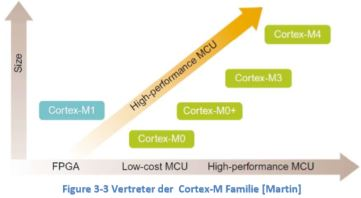
\includegraphics[width=\linewidth]{images/cortexmfam}
    
    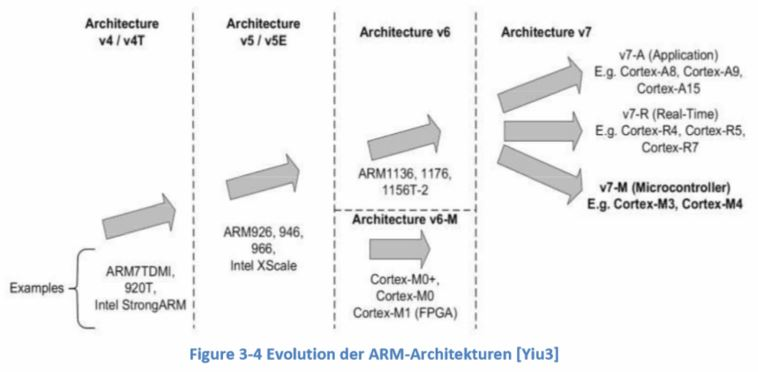
\includegraphics[width=\linewidth]{images/cortexmcomp}
\end{multicols}

\begin{multicols}{3}
    \textbf{Cortex-A}
    \begin{itemize}
        \item HighEnd Anwendungen und Betriebssysteme
        \item hohe Rechenleistung
        \item Chache Memory
    \end{itemize}
    
    \textbf{Cortex-R}
    \begin{itemize}
        \item Echtzeitfähigkeit
        \item hohe Zuverlässigkeit
        \item System on Chip (SOC) 
    \end{itemize}  
    
    \textbf{Cortex-M}
    \begin{itemize}
        \item Speziell für $\mu$ C-Markt
        \item Low Cost, Low Energy
        \item System on Chip (SOC) 
    \end{itemize}             
\end{multicols}

\subsubsection{Vorteile der Cortex-M-Prozessoren}
\begin{multicols}{2}
    \begin{itemize}
        \item Low Power
        \subitem < 200$\mu$ A / MHz
        \item Performance
        \subitem >1.25 DMIPS / MHz
        \item Energy Efficiency
        \subitem low Power, high performance
        \item Code Density
        \subitem Thumb 2 Befehlssatz
        \item Interrupts
        \subitem 240 Interrupts
        \item Easy of Use, C Friedly
        \item Scalability
        \item Debug Features
        \item Software portability and Reusebility
        \item OS Support
        \item Choices (Derivers, Tools, OS,..)    
    \end{itemize}
\end{multicols}
\clearpage 

\subsection{Cortex-M3/M4}
\begin{multicols}{2}
    \begin{itemize}
        \item Harvard Architecture
            \subitem $\rightarrow$  Zugriffe auf Instruktionen und Daten
            \subitem \qquad können gleichzeitig stattfinden
        \item Internal Bus Interconnect
            \subitem $\rightarrow$ mehrere Bus-Interface 
        \item Nested Interrupt Controller \textbf{(NVIC)}
        \item Standart Timer \textbf{(SYSTICK)}\\
        \textbf{Optional:}
        \item Memory Protection Unit \textbf{(MPU)}
        \item Floating Point Unit \textbf{(FPU)}
    \end{itemize}
\end{multicols}

\subsection{System-Komponenten}
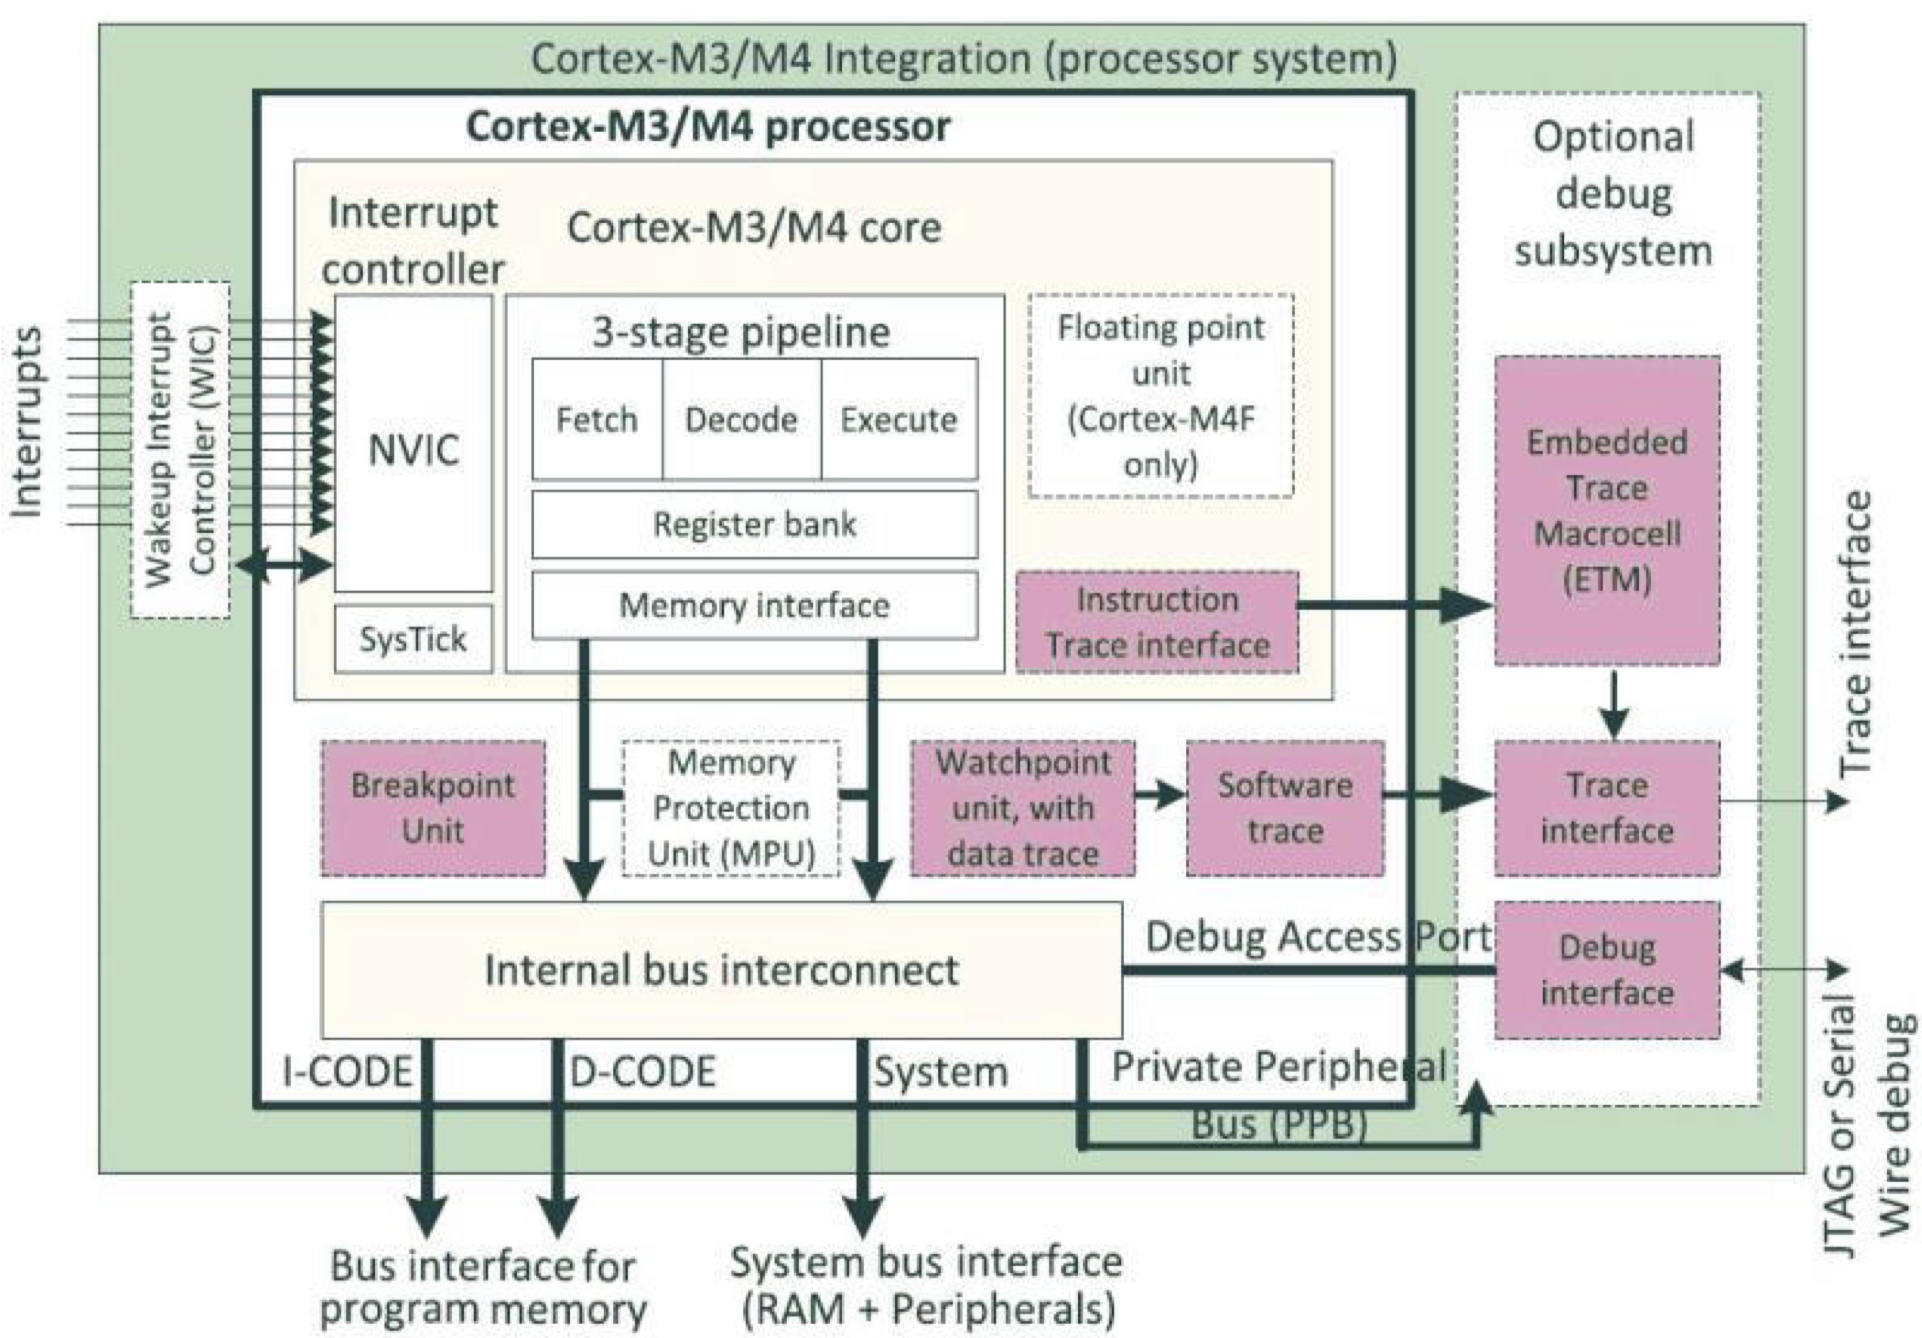
\includegraphics[width=13.5cm]{images/Blockdiagramm}
\begin{multicols}{2}
    \begin{minipage}{\linewidth}
        \subsubsection{NVIC}
        \begin{itemize}
            \item Non-Maskable Interrupt (NMI)
            \item Bis zu 240 externe Interrupts
            \item 8 bis 256 Prioritätslevel
        \end{itemize}
        $\rightarrow$ ISR benötigt 12 Taktzyklen\newline
        Siehe auch:\nameref{NVIC} S\pageref{NVIC}\\
    \end{minipage}

    \begin{minipage}{\linewidth}
        \subsubsection{WIC (Wakeup Interrupt Controller)}
        Für die Umsetzung von Low-Power-Modes.\newline
        Dadruch kann 99\% der Cortex M3-Prozessoren im Low-Power-Bereich arbeiten.
        \newline
        \newline
        Ist mit dem NVIC verknüpft und holt den Prozessor aus diesem Modus heraus, um auf einen Interrupt reagieren zu können\\
    \end{minipage}
    
    \begin{minipage}{\linewidth}
        \subsubsection{FPU - (nur Cortex M4!)}
        Mit der FPU lassen sich IEEE754 Signal Precision Floating-Point Operationen in sehr wenigen Takten ausführen\\
    \end{minipage}
    
    \begin{minipage}{\linewidth}
        \subsubsection{MPU}
        \begin{itemize}
            \item ermöglicht Zugriffsregel für den Privilieged Access und User Programm Access zu definieren
            \item $\rightarrow$ Wird eine Zugriffsrege verletzt erfolgt eine Exception-Regelung wodurch der Exceptrion Handler das Problem analysiert und ggf. beheben kann
            \item $\rightarrow$ Ausserdem ist es möglich gewisse Bereiche als read-only zu deklarieren
        \end{itemize}
    \end{minipage}
\end{multicols}

\begin{multicols}{2}
    \begin{minipage}{\linewidth}
        \subsubsection{SYSTICK}
        \begin{itemize}
            \item 24-Bit Countdown-Timer mit automatischer Relaod-Funktion
            \item Wird für einen periodischen Interrupt verwendet
        \end{itemize}
        Wenn der Zähler den Wert 0x000000, wird dies dem NVIC signalisiert und  der Reload-Wert wird aus dem Reload-Register gelesen.
    \end{minipage}
    \\
    \newline
    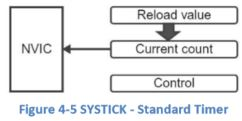
\includegraphics[width=6.5cm]{images/NVIC}\\
\end{multicols}
\clearpage
%============================================

\subsection{GNU-Tool-Chain Entwicklungsablauf}
\begin{multicols}{2}
    \begin{minipage}{\linewidth}
        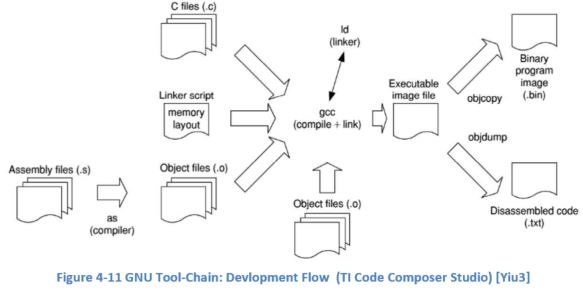
\includegraphics[width=\textwidth]{images/gnutoolchain}
        \begin{tabular}{|l|l|}
            \hline 
            \textbf{APSR}& Application Program Status Register \\ 
            \hline 
            \textbf{IPSR}& Interrupt Program Status Register \\ 
            \hline 
            \textbf{EPSR}& Execution Program Status Register \\ 
            \hline 
            \end{tabular}
        \subsubsection{SP-zugriffe (Assembler)}
        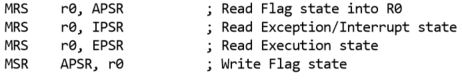
\includegraphics[width=\textwidth]{images/SPzugriffe}   
    \end{minipage}
    
    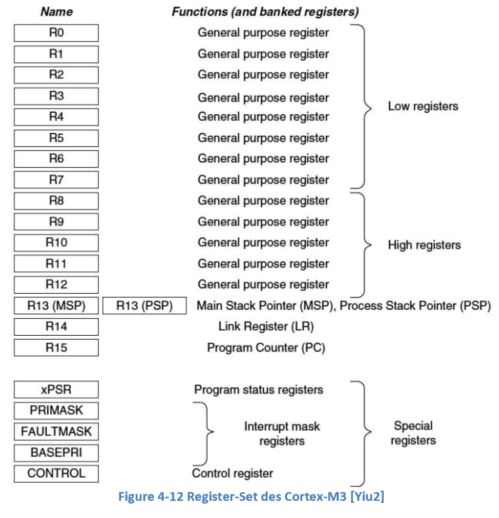
\includegraphics[width=0.5\textwidth]{images/gnutoolchain1}
\end{multicols}

\subsection{Programm Status Register}
\begin{minipage}{9cm}
	\begin{tabular}{|m{2cm}|m{6cm}|}
        \hline 
        \textbf{N}& Negativ \\ 
        \hline 
        \textbf{Z}& Zero  \\ 
        \hline 
        \textbf{C}& Carry/borrow  \\ 
        \hline 
        \textbf{V}& Overflow \\ 
        \hline 
        \textbf{Q}& Sticky saturation flag \\ 
        \hline 
        \textbf{ICI/IT}& Interrupt-Continauble Instruction(ICE) bits\\
                        & IF-THEN instruction status bit \\ 
        \hline 
        \textbf{T}& Thumb state, always 1; Trying to clear this bit will caus a fault exception \\ 
        \hline 
        \textbf{Exception number}& Indicates which exception the processor is handling \\ 
        \hline 
    \end{tabular} 
\end{minipage}
%
\begin{minipage}{0.5cm}
	\-\
\end{minipage}
%
\begin{minipage}{9cm}
	\subsubsection{Q-Flag}
This flag is set to 1 if any of the following occurs:
\begin{itemize}
    \item Saturation of the addition result in a \textit{QADD or QDADD} instruction
    \item Saturation of the subtraction result in a \textit{QSUB or QDSUB} instruction
    \item Saturation of the doubling intermediate result in a \textit{QDADD or QDSUB} instruction
    \item Signed overflow during an \textit{SMLA<x><y> or SMLAW<y>} instruction
\end{itemize}
The Q flag is sticky in that once it has been set to 1, it is not affected by whether subsequent calculations saturate and/or overflow.\newline
\textbf{An example:}\newline
\textit{0x70000000 + 0x70000000} would become \textit{0xE0000000}, but since qadd is saturating, the result is saturated to \textit{0x7FFFFFFF} (the largest positive 32-bit integer) and the Q flag is set.
\end{minipage}

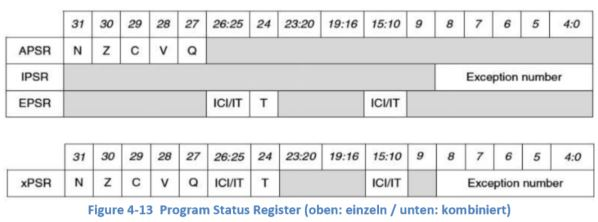
\includegraphics[width=14.5cm]{images/programstatusregister}

\clearpage
\subsection{Stack}
\begin{minipage}{9cm}
	\subsubsection{Eigenschaften}
	\begin{itemize}
            \item Temporäre Zwischenspeicherung von Daten während der ausführung einer Funktion
            \item Übergabe von Informationen an Funktionen oder Subroutinen
            \item Speichern von lokalen Variabeln
            \item Erhalten von Prozessor-Status und Register-Werten, während Exceptions oder Interrupts ausgefüht werden
            \item PUSH-POP-Instruktionen werden ausgeführt
            \item LIFO-Prinzip(Last In, First Out)
        \end{itemize}
\end{minipage}
%
\begin{minipage}{0.5cm}
	\-\
\end{minipage}
%
\begin{minipage}{9cm}
	 \subsubsection{Main-Stack-Pointer (MSP)}
        \begin{itemize}
            \item Standard Stack Pointer nach einem Reset
            \item Innerhalb von Exception-Interrupt-Handler wird immer der MSP benutzt!
            \end{itemize}
        \subsubsection{Prozessor-Stack-Pointer (PSP)}
        \begin{itemize}
            \item Alternativer Stackpointer
            \item Wird nur im Thread-Mode verwendet
            \subitem $\rightarrow$ bei embedded OS-System
        \end{itemize}   

\end{minipage}

\subsubsection{PUSH-POP Operationen}
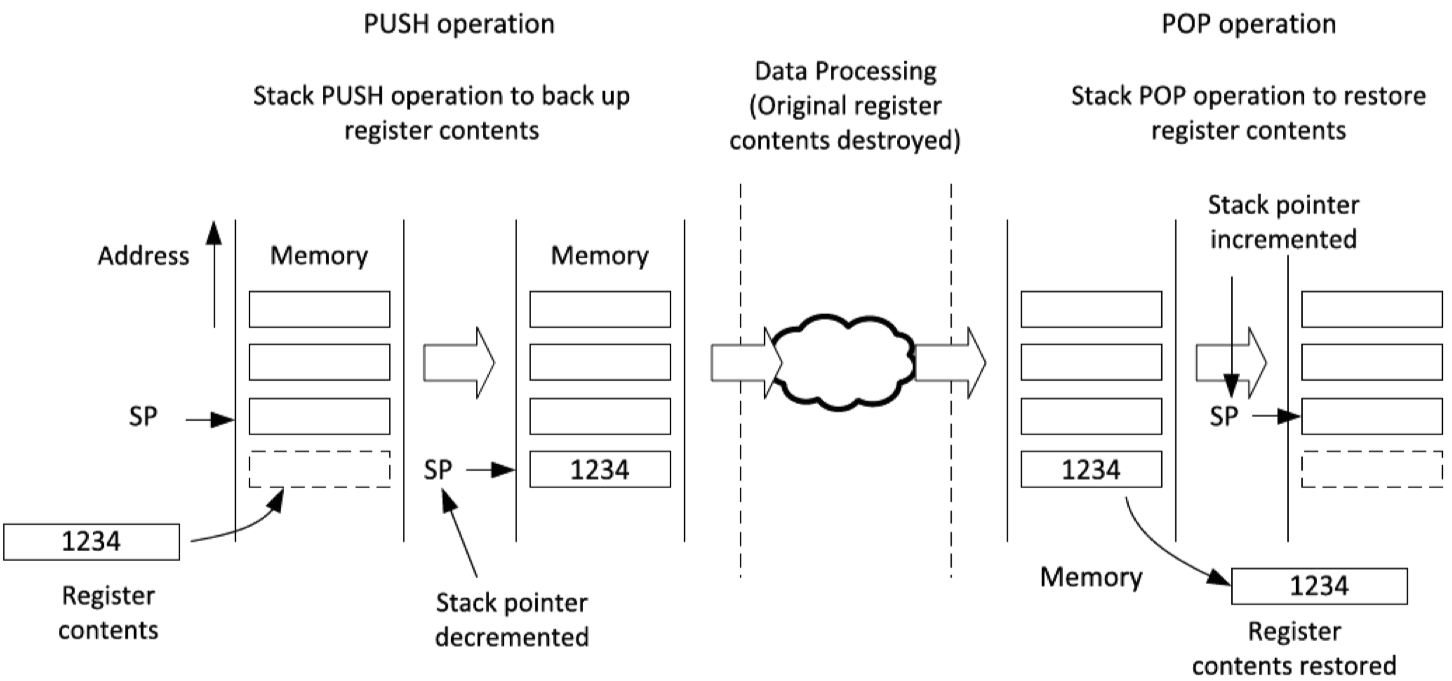
\includegraphics[width=16cm]{images/Stack}

Der Stack wird von der h"ochsten Adresse aus gef"ullt, das heisst das bei einer PUSH-Operation der Stack-Pointer dekrementiert wird. Es gibt auch kombinierte PUSH/POP Operationen. Die wohl wichtigste ist die POP/Return Operation, bei welcher das Link-Register (LR) beim PUSH auf den Stack gelegt wird und bei der POP-Operation direkt in den Programm-Counter (PC) geschrieben wird. Da alle Register in der Registerbank 32-Bit breit sind, wird der Stack-Pointer immer eine \textit{4-Byte aligned Adresse} enthalten.










